% -*- root: ../../main.tex -*
%!TEX root = ../../main.tex
% vim:textwidth=80 fo=cqt conceallevel=0


It is  important to provide the  contextual setting for this  layer optimisation
work since it is nestled deep  within the broader horizon of electric drivetrain
optimisation. \Cref{fig:fig_PowertrainSchematic}  provides a  graphical overview
depicting the hierarchical architecture of  a typical \gls{xeV} powertrain, from
the  system level  down to  a  single electrochemical  layer. The  rest of  this
section describes the scope of this  layer optimisation work and its integration
into this  overall architecture. A further  set of assumptions that  were deemed
inopportune to be discussed  in \cref{subsec:layeroptassumptions}, is introduced
at apropos junctures  throughout this narrative. The overall  architecture of an
\gls{xeV}  powertrain  can  be  studied through  a  systematic,  hierarchical
evaluation at ---
\begin{enumerate*}[label=\itshape\alph*\upshape)]
    \item the system-level,
    \item the pack-level, and
    \item the cell-level.
\end{enumerate*}

\begin{figure}[!bp]
    \begin{minipage}[t]{\textwidth}
        \centering
        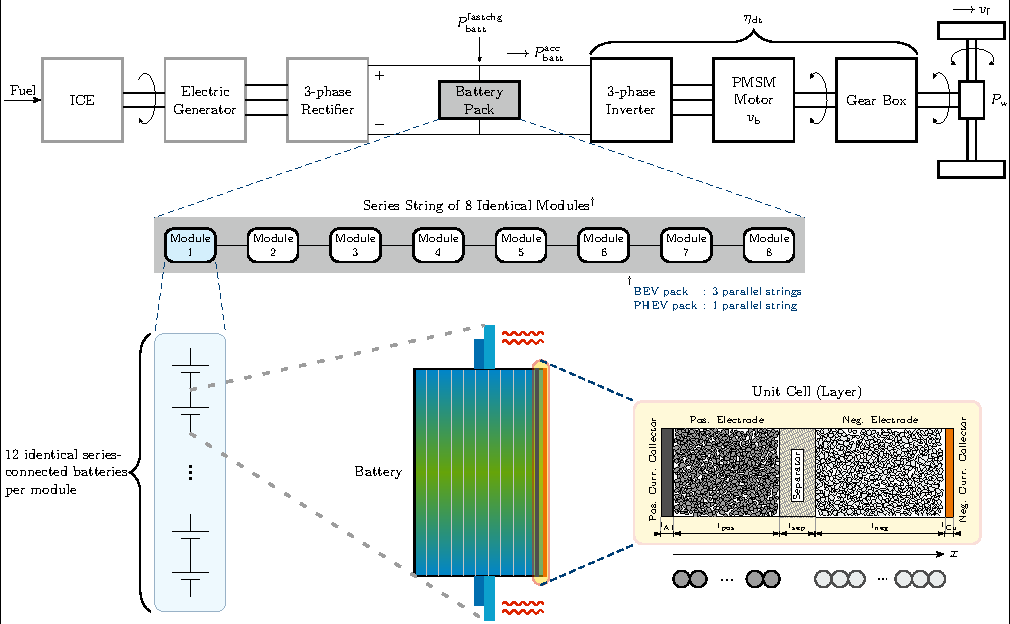
\includegraphics[width=\textwidth]{hierarchical_powertrain_to_cell_layer.pdf}
        \captionsetup{labelsep=note}
        \caption
        [%
        Vehicle-to-cell hierarchical overview of an electrified powertrain architecture
        ]%
        {%
            Schematic depicting the vehicle-to-cell hierarchical overview of
            a typical electrified powertrain architecture. This represents the
            system-level context within which the proposed layer optimisation framework
            has been developed. Two \glsfmtshort{xeV} powertrains ---
            \begin{enumerate*}[label=\itshape\alph*\upshape)]
                \item a \gls{bev}, and
                \item a series \gls{phev}
            \end{enumerate*}
            are chosen as examples to demonstrate how the methodology facilitates
            common module designs for such battery packs.
        }%
        \label{fig:fig_PowertrainSchematic}
        \mpfootnotes[1]
        \footnote{This figure was created by \mbox{Krishnakumar Gopalakrishnan} who
            asserts copyright, with intellectual contributions from and the right to
        use asserted by \mbox{Ian D.\ Campbell}.}
    \end{minipage}
\end{figure}

\subsection{System-level --- vehicular platforms}

The top row of  \cref{fig:fig_PowertrainSchematic} represents the typical layout
of a \emph{series}-hybrid powertrain~\cite{Maksimovic2012}. Partly to supply the
mechanical  power and/or  partly  to  charge the  battery  during propulsion,  a
downsized \gls{ice} is  employed. The \gls{ice} is coupled to  the pack's DC bus
through  a  generator  and  three-phase  rectifier.  While  tackling  the  power
handling  requirements,  irrespective  of  whether  a  \gls{bev}  or  \gls{phev}
powertrain is  being considered, the  cells in the pack  are to be  designed for
the  worst-case operating  scenario \ie~without  any power  support from  the
\gls{ice}. This implies that all discharge  simulations of the \gls{phev} are to
be conducted with  the powertrain operating in all-electric mode  resulting in a
net charge-depletion. The only distinction is that the \emph{magnitude} of power
to  be handled  by the  pack in  this worst  case scenario  is vastly  different
between the \gls{bev} and \gls{phev}  cases. This allows for some simplification
as explained  below and  helps to  narrow down the  scope of  the problem  to be
tackled.

Omitting the  components to the  left of the  battery pack (represented  as text
boxes with light grey border) shall render a powertrain corresponding to that of
a  \gls{bev}.  The proposed  layer  optimisation  methodology is  developed  and
presented in the context of this  \gls{bev} powertrain. However, being a modular
framework, the optimisation methodology may  be readily extended to a \gls{phev}
powertrain.

As  shown   in  \cref{fig:fig_PowertrainSchematic},  the   \gls{bev}  powertrain
typically comprises of ---
\begin{enumerate*}[label=\itshape\alph*\upshape)]
    \item a battery pack,
    \item a three phase inverter,
    \item a \gls{pmsm},
    \item a gearbox for  torque multiplication, and
    \item the rest of the  powertrain  (differential shaft  and driven  wheels).
\end{enumerate*}
Considering the  worst-case scenarios, the  power to  be handled by  the battery
pack arises due to  ---
\begin{enumerate*}[label=\roman*)]
    \item fast charging from  the mains~$P^\text{fastchg}_\text{batt}$~(charge), or
    \item acceleration  from standstill~$P^\text{acc}_\text{batt}$~(discharge).
\end{enumerate*}
The   acceleration  power   is  computed   from  the   power  required   at  the
wheels~$P_\text{w}$.  The   details  of  this  calculation   is  presented  in
\cref{sec:accpathway}.  The  sign  convention  used  in  this  chapter  is  that
the  charging power  is positive  (and  consequently, the  discharging power  is
negative).

\subsection{Pack-level --- strings, modules \& cells}\label{sec:packlevelhierarchy}

Delving  into the  battery pack  under  consideration, this  thesis considers  a
standard  modular  layout wherein  the  \gls{phev}  pack  has one  string  while
the  \gls{bev}  pack  has  three  parallel strings in congruence with a
contemporary pack design. Within  each  string,  both vehicular  platforms
employ  8~series-connected  modules.  Taking cognisance  of the  benefits  of
common  module  design,  identical  pack modules  are  assumed across  both 
\gls{xeV}  platforms  which  is  then  extrapolated  to  impose  a stronger 
condition  of  identical  geometry  for  the  constituent  cells  (see
\cref{subsec:layeroptassumptions}). The  exterior dimensions of the  pouch cells
under consideration are listed in \cref{tbl:lcoSimParamslayeropt}.

Each module consists  of 12~identical series-connected cells  denoted by battery
circuit symbols (cyan-filled  blocks in \cref{fig:fig_PowertrainSchematic}). The
\gls{phev} pack is  smaller and consists of only \ordfrac{1}{3}  of the cells in
the \gls{bev} pack. Assuming that the \gls{bev} pack consists of a \mbox{96S-3P}
cell  assembly,  this implies  that  the  \gls{phev}  pack  shall conform  to  a
\mbox{96S-1P} layout. The DC~bus voltage is unaltered since both packs have same
amount of  series cells. The power  flow is assumed to  be uniformly distributed
across all  the cells within  the pack(s). At first,  the power required  at the
terminals of the  pack is computed. From this, a  first-order design ball-parking
of the layers of the cell is made through a single cell simulation. This process
enables reduced simulation run-time with the conditions of one cell assumed to be
representative of all cells in the pack.


% At a  high-level, the  essence of  the layer  optimisation methodology  can be
% distilled down to the following sequence.

While the aforementioned assumption of identical cell conditions across the pack
seems infeasible at first glance, three careful considerations have been made to
justify  this assumption.  Firstly,  power  (and not  current)  is  used as  the
stimulus to the cell. This  implies that, despite the \emph{parallel} connection
of cells  (in groups of three  cells within each module),  each cell experiences
the same  power. Even  across parallel-connected strings,  the power  handled by
each cell shall be the same.  This necessitates the modification of the standard
\gls{dfn}  model in  order to  accommodate power  inputs which  is discussed  in
\cref{sec:innatepowerinput}. Secondly,  although the current  in all cells  of a
\emph{series}  string remain  the same  (by virtue  of Kirchoff's  current law),
their  terminal voltage  levels could  drift away  from each  other and  becomes
unbalanced over  time~\cite{Andrea2010}. This naturally raises  questions on the
assumption  of  identical  conditions  for  all  cells.  However,  this  voltage
unbalance is mitigated with the help of modern \glspl{bms} that employ balancing
techniques  such as  passive  bleeder resistors  or  sophisticated active  dc/dc
converters. Yet another adverse effect that  poses a threat to the assumption of
identical  conditions  is  the  uneven distribution  of  cell  temperatures.  In
automotive packs employing natural convection, cells that are physically located
innermost in  the string tend  to get hotter  than the outermost  cells. Through
good thermal management  design \eg~forced cooling through  circulation of the
coolant through conduits grooved into the pack, thermal balance may be achieved.
Therefore,  it  can be  argued  that,  when  operating  in a  well-designed  and
controlled environment,  cell-to-cell deviations  are minimised.  This justifies
the  global representation  of  all  cells in  the  pack  through a  single-cell
simulation, although modifications to the  simulation model are deemed necessary
to facilitate power inputs and is discussed in \cref{sec:innatepowerinput}.


% Since  thermal effects  need to  be considered  for robust  cell design,

\subsection{Cell-level --- layers, cooling, electrochemical \& thermal models}\label{sec:celllevelxeVinfo}

The    illustration    at     the    centre    of    the     bottom    row    in
\cref{fig:fig_PowertrainSchematic} shows  a schematic  representation of  a cell
arranged within  each module. In practice,  the physical layout of  cells within
a  module  is  slightly  more  complex.  For  instance,  a  typical  arrangement
consists  of  groups   of  3~parallel  cells.  However,   the  illustration  in
\cref{fig:fig_PowertrainSchematic}  suffices to  explain  the necessary  details
required for the specific task at hand.

Each cell in the pack consists of a number of identical layers~$n$. The words
`layer' and `unit-cell' are used interchangeably in this thesis to denote a
single basic electrochemical unit consisting of ---
\begin{enumerate*}[label=\roman*)]
    \item a~positive current-collector,
    \item a~positive electrode region,
    \item a~separator material,
    \item a~negative electrode region, and
    \item a~negative current-collector~(see \cref{fig:chargetransferprocess}).
\end{enumerate*}
Particular attention is called out in  regard to the distribution of temperature
within  the cell.  In  the schematic  of \cref{fig:fig_PowertrainSchematic}  the
shading scheme  is such that greener  tints represent the hotter  regions of the
cell while bluer tints represent colder regions. The temperature distribution
within the cell as indicated by this shading scheme is consistent with that
reported in literature~\cite{Veth2014,Bazinski2014,Zhao2018}. Furthermore, heat
exchange with the surroundings is also graphically  illustrated through cooling
plates mounted at the tabs  of the cell. This  highlights the specific type  of
cooling assumed \viz~\emph{tab-cooling}  as  opposed to  conventional 
\emph{surface-cooling} historically employed for automotive applications. The
assumption of tab-cooling is an  essential requirement for  upholding the 
validity of the  proposed layer optimisation scheme, and therefore warrants
further justification.

An  experimental  study  by   Hunt~\etal~\cite{Hunt2016}  compared  tab  cooling
of  cells  against conventional  surface  cooling.  It  was found  that  \approx
\SI{8}{\percent} increase in the usable  capacity of pristine cells was achieved
with tab cooling relative to that  achieved with surface cooling. Secondly, with
surface  cooling, the  loss rate  of usable  capacity over  thousand cycles  was
nearly thrice of that with tab cooling.  This implies that using tab cooling can
potentially help to extend the lifetime of  the pack by three times. Thirdly, at
higher discharge rates,  surface cooling resulting in a loss  of usable capacity
of \SI{9.2}{\percent} compared  to just \SI{1.2}{\percent} for  tab cooling. The
simulations  discussed  as  part  of  the  optimisation  framework  reported  in
\cref{sec:layeroptframework} are intended to  obtain robust cell designs capable
of handling  worst-case power inputs.  In these  scenarios, tab cooling  is more
appropriate.  Therefore,  this author  has  no  qualms about  recommending  this
specific cooling mechanism  to be used in conjunction with  the results reported
(see  \cref{sec:resultslayeropt}) by  applying the  proposed layer  optimisation
scheme.

Apart  from  its  aforementioned  beneficial   effects  on  cell  longevity  and
performance,  with the  integral  assumption  of tab  cooling,  there exists  an
important side effect  that affects the very  core of the numerics  of the layer
optimisation methodology.  Carefully examining the  shading scheme used  for the
schematic  in the  centre-bottom  of  \cref{fig:fig_PowertrainSchematic}, it  is
clear that  at any vertical  co-ordinate in space  within the cell,  the shading
across the entire cell width remains  uniform throughout. This implies that each
layer  along  a  one-dimensional  cross-section  of the  cell  is  at  the  same
temperature. Based  on the inferences from  Hunt~\etal~\cite{Hunt2016}, with tab
cooling, only  small thermal gradients are  induced in the planar  direction. In
this unique scenario,  the thermal effects within the cell  are not large enough
to warrant a detailed numerical discretisation.  On the other hand, ignoring the
temperature distribution  of the  cell shall  not lead  to robust  cell designs,
especially given  that design simulations  typically involve high  magnitudes of
power.

In  situations akin  to  aforementioned circumstances,  a  lumped thermal  model
of  the cell  has  been  recommended by  Pals  and Newman~\cite{Pals1995}.  This
represents a good trade-off between accuracy and simplicity and hence, is deemed
to  be  appropriate for  this  design  application.  A  suitable value  for  the
convective heat transfer  coefficient~$h$ (see \cref{tbl:lcoSimParamslayeropt}),
comparable  to the  typical  magnitudes in  forced air  convection,  is used  to
represent the heat transfer from the  cell to the environment. The heat exchange
area is the combined  surface area of the two cooling tabs  that are situated at
either end  of the  cell. The temperature  of the coolant  (a thermal  `sink' in
thermodynamic  terminology) is  denoted by~$T_\text{sink}$.  In this  work, this
ambient temperature is held constant during  the course of a simulation run, but
is allowed  to change to  different constant  values between set  of simulations
as  per relevant  vehicle  testing  standards. The  details  of  this aspect  is
discussed  in  \cref{sec:layeroptframework}.  The  material  properties  of  the
constituent components  of each layer  coupled with  the total number  of
layers are used  to determine  the  lumped  mass  and specific  heat  capacity 
of  the  pouch cell.  These  computations  are  discussed  in 
sections~\ref{sec:massofonecell} and~\ref{sec:spheat} respectively. The 
assumption of tab cooling  thus leads to this qualitative  description of  the
lumped  thermal model to  be used  for the design simulations.  Further
quantification by  way of relevant  model equations and  the computation  of 
the constituent  parameters of  the  thermal model  is embedded as an integral
aspect of  the layer optimisation framework and shall be presented in
\cref{sec:spheat}.

As a final observation, all layers  within the cell are electrically in parallel
which implies that their terminal voltages are identical. The current (or power)
at the  cell terminals is  shared equally  among each layer.  The aforementioned
considerations have important  ramifications on the cell modelling  and helps to
drastically  simplify  it. Specifically,  these  considerations  imply that  the
electrochemical  performance  of any  one  layer  is  identical to  every  other
layer.  Therefore,  in conjunction  with  a  lumped  thermal model,  a  standard
\gls{p2d}  discretisation  of  the  \gls{dfn}  model  suffices  to  capture  the
electrochemical behaviour of  the entire cell. The  bottom-right illustration of
\cref{fig:fig_PowertrainSchematic} presents a  one-dimensional discretisation of
the  cell layer  across its  thickness. The  spheres along  the axial  direction
represent computational nodes  wherein the solid-phase diffusion  equation is to
be solved  (see \cref{sec:dfnmodel} for a  brief overview). It is  this standard
\gls{dfn}  model,  suitably  amended  to  accept  power  inputs,  that  will  be
the  backbone of  the  electrochemical  aspects of  the  design simulation.  The
electrochemical model shall be strongly coupled  in a bidirectional sense to the
lumped thermal model  \ie~the temperature of the cell  shall influence various
cell parameters  (see \cref{tbl:lcoSimParamslayeropt}) while  the overpotentials
and currents in  the cell shall play a  role in the rate of  heat generation and
cell temperature simultaneously.

Thus, through a  systematic set of simplifying assumptions  that are justifiable
in a real-world  design, the system-level requirements at the  pack-level can be
suitably  scaled  down  to  power-density  inputs at  the  layer  level.  Having
established the  contextual setting and  scope of  this work within  the broader
landscape of drivetrain  optimisation, it is now possible to  proceed to the set
of numerical enhancements  required to be incorporated into  the \gls{dfn} model
to handle the specific requirements of this layer optimisation task.

